\documentclass[a4paper,12pt]{article}

%%% Работа с русским языком
\usepackage{cmap}					% поиск в PDF
\usepackage{mathtext} 				% русские буквы в формулах
\usepackage[T2A]{fontenc}			% кодировка
\usepackage[utf8]{inputenc}			% кодировка исходного текста
\usepackage[english,russian]{babel}	% локализация и переносы
\usepackage{xcolor}
\usepackage{hyperref}
 % Цвета для гиперссылок
\definecolor{linkcolor}{HTML}{799B03} % цвет ссылок
\definecolor{urlcolor}{HTML}{799B03} % цвет гиперссылок

\hypersetup{pdfstartview=FitH,  linkcolor=linkcolor,urlcolor=urlcolor, colorlinks=true}

%%% Дополнительная работа с математикой
\usepackage{amsfonts,amssymb,amsthm,mathtools} % AMS
\usepackage{amsmath}
\usepackage{icomma} % "Умная" запятая: $0,2$ --- число, $0, 2$ --- перечисление

%% Номера формул
%\mathtoolsset{showonlyrefs=true} % Показывать номера только у тех формул, на которые есть \eqref{} в тексте.

%% Шрифты
\usepackage{euscript}	 % Шрифт Евклид
\usepackage{mathrsfs} % Красивый матшрифт

%% Свои команды
\DeclareMathOperator{\sgn}{\mathop{sgn}}

%% Перенос знаков в формулах (по Львовскому)
\newcommand*{\hm}[1]{#1\nobreak\discretionary{}
{\hbox{$\mathsurround=0pt #1$}}{}}
% графика
\usepackage{graphicx}
\graphicspath{{pictures/}}
\DeclareGraphicsExtensions{.pdf,.png,.jpg}
\author{Бурмашев Григорий, БПМИ-208}
\title{Матан, дз -- 12}
\date{\today}
\begin{document}
\maketitle 
\section*{Номер 1}
\[
(x^2 + y^2)^3 = x^4y
\]
Переходим в полярные координаты:
\[
(r^2)^3 = r^5 \cos^4 \varphi \sin \varphi
\]
\[
r = \cos^4 \varphi \sin \varphi 
\]
Смотрим на график:
\begin{center}
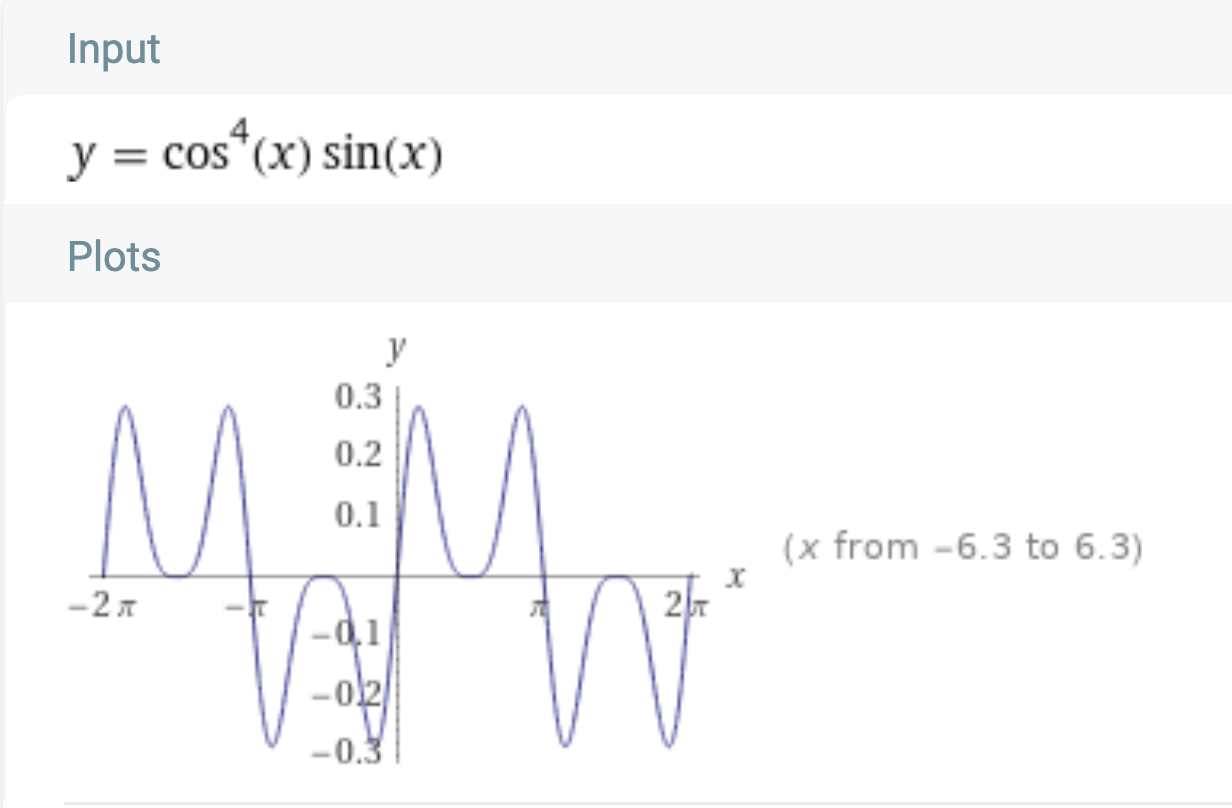
\includegraphics[scale=0.4]{1.png}
\end{center}
У нас $r > 0$, значит интервал от $\pi$ до $2\pi$ нас не интересует, будем брать от 0 до $\pi$
\[
S = \int_0^{\pi} d\varphi \int_0^{\cos4 \varphi \sin \varphi} 1\cdot  r dr =\int_0^{\pi} d\varphi \int_0^{\cos4 \varphi \sin \varphi} 1\cdot  r dr = \int_0^{\pi} d\varphi \left(\frac{r^2}{2}\right) \Bigg|^{{\cos^4 \varphi \sin \varphi}}_{0}
\]
\[
= \int_0^{\pi} d\varphi \left(\frac{\cos^8 \varphi \sin^2 \varphi }{2}\right) =  \frac{1}{2} \int_0^{\pi}  \left(\cos^8 \varphi \sin^2 \varphi\right)d\varphi = ( \times ) 
\]
 Такой интеграл особо не посчитаешь, вольфрам выдает какую-то странную  рандомную формулу, поэтому буду в тупую раскладывать по формулам из школы:
\[
\cos^8 x \sin^2 x = \cos^7 x \sin x \cdot (\cos x \sin x) = \cos^7 x \sin x  \left(\frac{1}{2}\sin2x\right) = cos^6x \left(\frac{1}{2}\sin2x\right) \left(\frac{1}{2}\sin2x\right) = 
\]
\[
=
\frac{1}{4}  (\cos^2 x)^3\sin^2 2x  = \frac{1}{4} \left(\frac{1}{2}(1 + \cos 2x)\right)^32 \sin^2 x = \frac{1}{4} \cdot \frac{1}{8} \left(1 + \cos2x \right)^3 \sin^2 2x = 
\]
\[
=
\frac{1}{32} (1 + \cos 2x)^3 \sin^2 2x = \frac{1}{32} \left(\cos^3 2x + 3\cos^2 2x +3 \cos 2x + 1 \right) \sin^2 2x = 
\]
\[
=
\frac{1}{32} \left(\cos^3 2x \sin^2 2x + 3\cos^2 2x \sin^2 2x + 3\cos 2x \sin^2 2 x + \sin^2 2x \right)
\]
Тогда наш интеграл принимает вид:
\[
(\times) =  \frac{1}{64} \int_0^{\pi} \left(\cos^3 2\varphi \sin^2 2\varphi + 3\cos^2 2 \varphi\sin^2 2 \varphi  + 3\cos 2 \varphi \sin^2 2 \varphi + \sin^2 2 \varphi \right) d \varphi 
\]
Посчитаем по отдельности и потом сложим как сумму:

\begin{itemize}
\item \[
\int \cos^3 2 \varphi \sin^2 2 \varphi d \varphi = \begin{vmatrix}
u = \sin 2 \varphi \\
du = 2 \cos 2 \varphi d \varphi \\
d \varphi = \frac{du}{2 \cos 2 \varphi}
\end{vmatrix} = \frac{1}{2} \int \cos^3 2 \varphi \cdot u^2 \frac{du}{\cos 2 \varphi}  = \frac{1}{2} \int  (1-u^2) u^2 du = 
\]
\[
=
\frac{1}{2 } \int (u^2 - u^4) du = \frac{1}{2} \left(\frac{\sin^3 2 \varphi}{3} - \frac{\sin^5 2 \varphi}{5}\right)
\]
\[
\int_0^{\pi} \cos^3 2 \varphi \sin^2 2 \varphi d \varphi  = \frac{1}{2} \left(\frac{\sin^3 2 \varphi}{3} - \frac{\sin^5 2 \varphi}{5}\right) \Bigg|^{\pi}_0 = \frac{1}{2}(0 - 0) = 0
\]
\item
\[
\int \cos^2 (2 \varphi) \sin^2 (2 \varphi)d \varphi = \int \frac{1}{4} \sin^2 4 \varphi d \varphi  = \frac{1}{4} \int \sin^2 4 \varphi d \varphi  = \frac{1}{4} \int \frac{1 - \cos 8 \varphi}{2} d \varphi = 
\]
\[
=
\frac{1}{8} \int 1 - \cos 8\varphi d \varphi = \frac{1}{8} \varphi - \frac{1}{8} \cdot \frac{1}{8} \sin 8 \varphi 
\]
\[
3\int_0^{\pi} \cos^2 (2 \varphi) \sin^2 (2 \varphi)d \varphi = 3 \left(\frac{1}{8} \varphi - \frac{1}{64} \sin 8 \varphi \right) \Bigg|^{\pi}_0 = 3\left(\frac{\pi}{8} - 0\right) = \frac{3\pi}{8}
\]
\item
\[
\int \cos 2 \varphi \sin^2 2 \varphi d \varphi =\begin{vmatrix}
u = \sin 2 \varphi \\
du = 2 \cos 2 \varphi d \varphi
\end{vmatrix}= \frac{1}{2} \int u^2 du = \frac{1}{2} \cdot  \frac{u^3}{3} = \frac{1}{6} \sin^3 2\varphi 
\]
\[
3\int_0^{\pi} \cos 2 \varphi \sin^2 2 \varphi d \varphi = 
3 \cdot \left( \frac{1}{6} \sin^3 2 \varphi \right)\Bigg|^{\pi}_0 = 3 \cdot (0 - 0) = 0
\]
\item
\[
\int \sin^2 2 \varphi d \varphi = \int \frac{1 - \cos 4 \varphi}{2} d \varphi  = \frac{1}{2} \int (1 - \cos 4 \varphi) d \varphi = \frac{1}{2} \varphi - \frac{1}{8} \sin 4 \varphi 
\]
\[
\int_0^{\pi} \sin^2 2 \varphi d \varphi  = \left( \frac{1}{2} \varphi - \frac{1}{8} \sin 4 \varphi \right) \Bigg|^{\pi}_0 = \frac{\pi}{2} - 0 = \frac{
\pi}{2}
\]
Возвращаемся к исходному интегралу:
\[
(\times) = \frac{1}{64} \left(0 + \frac{3\pi}{8} + 0 + \frac{\pi}{2}\right) = \frac{7\pi}{512}
\]
\begin{center}
\textbf{Ответ: } 
\[
\frac{7\pi}{512}
\]
\end{center}
\end{itemize}
\clearpage
\section*{Номер 2}
\[
2z =  x^2 + y^2, x^2 + y^2 + z^2 \leq 4z
\]
Имеем:
\[
z = \frac{x^2+y^2}{2}
\]
Неравенство будем рисовать как шар:
\[
x^2 + y^2 + z^2 = 4z
\]
Пересечем наши условия:
\[
\begin{cases}
2z = x^2 + y^2 \\
x^2 + y^2 + z^2 = 4z
\end{cases}
\]
\[
2z + z^2 = 4z
\]
\[
z^2 = 2z
\]
\[
z(z - 2) = 0
\]
\[
z = 0 , x^2 + y^2 = 0
\]
\[
z = 2, x^2 + y^2 =4 
\]
Графичек для понимания:
\begin{center}

\includegraphics[scale=0.3]{2.png}
\end{center}
На семе вывели формулу площади, у нас множество $D$ задается как $x^2 + y^2 \leq 4$, формула:
\begin{center}
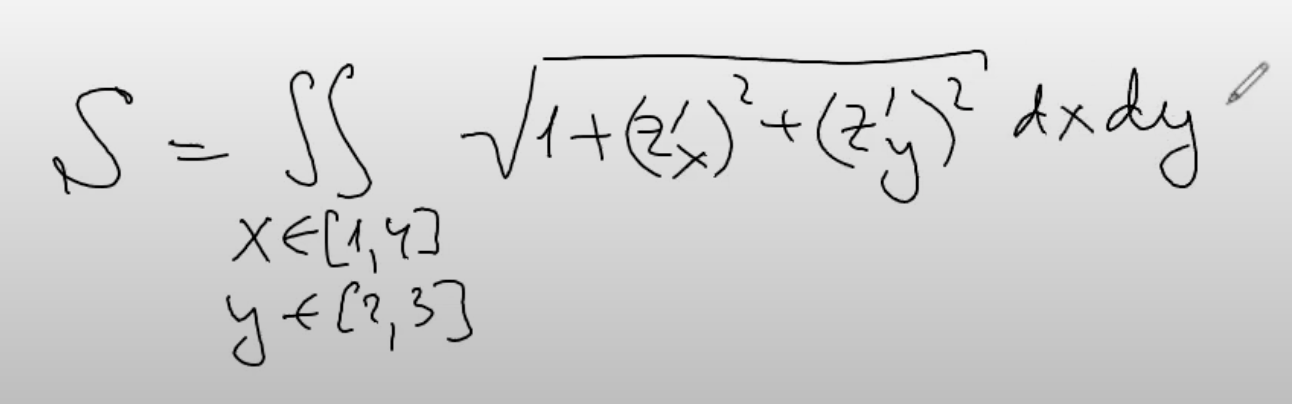
\includegraphics[scale=0.4]{3.png}
\end{center}
Итого имеем площадь:
\[
S = \iint\limits_{x^2 + y^2 \leq 4} \sqrt{1 + \frac{2x^2}{2} + \frac{2y^2}{2}} dx dy =  \iint\limits_{x^2 + y^2 \leq 4} \sqrt{1 + x^2 + y^2} dx dy = (\times)
 \]
Перейдем в полярные координаты: $x^2 + y^2$ удобно превратится в $r^2$:
\[
(\times) = \int_0^{2\pi} d \varphi \int_0^2 \sqrt{1+r^2} r dr = \begin{vmatrix}
u = r^2 + 1 \\
du = 2rdr \\
dr = \frac{du}{2r}
\end{vmatrix}
=
\int_0^{2\pi} d \varphi \frac{1}{2} \int_1^5 \sqrt{u}du  = \int_0^{2\pi} d \varphi \frac{1}{2}\frac{2u^\frac{3}{2}}{3} \Bigg|^5_1 =
\]
\[
= \int_0^{2\pi}  \frac{1}{2}\left( \frac{2 \cdot 5^\frac{3}{2}}{3} - \frac{2 \cdot 1}{3}  \right) d\varphi= \pi \left(\frac{10\sqrt{5} - 2}{3}\right)
\]
\begin{center}
\textbf{Ответ: } 
\[
 \pi \left(\frac{10\sqrt{5} - 2}{3}\right)
\]
\end{center}
\end{document}
